\documentclass[conference]{IEEEtran}
\IEEEoverridecommandlockouts
% The preceding line is only needed to identify funding in the first footnote. If that is unneeded, please comment it out.
\usepackage{hyperref}
\usepackage{cite}
\usepackage{amsmath,amssymb,amsfonts}
\usepackage{algorithmic}
\usepackage{graphicx}
\usepackage{textcomp}
\usepackage{xcolor}

\def\BibTeX{{\rm B\kern-.05em{\sc i\kern-.025em b}\kern-.08em
    T\kern-.1667em\lower.7ex\hbox{E}\kern-.125emX}}
\begin{document}

\title{Documentation of Fresh fruit detection AI}

\author{
\IEEEauthorblockN{1\textsuperscript{st} Bernard Swanepoel}
\IEEEauthorblockA{Faculty of Natural\\
and Agricultural Sciences\\
North-West University\\
39909476\\
Email: 39909476@mynwu.ac.za}
\and
\IEEEauthorblockN{2\textsuperscript{nd} Ashton du Plessis}
\IEEEauthorblockA{Faculty of Natural\\
and Agricultural Sciences\\
North-West University\\
34202676\\
Email: 34202676@mynwu.ac.za}
\and
\IEEEauthorblockN{3\textsuperscript{rd} Nico Deng}
\IEEEauthorblockA{Faculty of Natural\\
and Agricultural Sciences\\
North-West University\\
33700710\\
Email: 33700710@mynwu.ac.za}
}
\maketitle

\begin{abstract}
This paper presents a convolutional neural network (CNN) model and a mobile application for classifying fresh and rotten fruits. The CNN model is designed to distinguish between fresh and rotten apples, bananas, and oranges using image data. The model architecture consists of multiple convolutional layers, batch normalization, dropout, and fully connected layers. The training process utilizes data augmentation techniques, such as random horizontal flipping and normalization, to enhance the model's performance. The model is trained on a dataset of fruit images and evaluated for its classification accuracy. Additionally, a mobile application is developed to integrate the trained model for real-time fruit classification. The application allows users to load fruit images, preprocess them, and obtain predictions from the CNN model. The predicted class, either fresh or rotten fruit, is displayed to the user along with the corresponding image. The proposed system demonstrates the potential for automating fruit quality assessment and facilitating efficient sorting and grading processes in the agricultural industry or daily use.
\\
\end{abstract}

\begin{IEEEkeywords}
Rectified Linear units, Deep Learning,
Neural Networks, Supervised Learning, Structured Learning
\end{IEEEkeywords}

\section{Introduction}

It is known that some individuals might find it difficult to identify whether fruit is fresh or rotten. This can be due to various factors such as visual impairments, lack of experience, or subtle signs of decay that are not easily detectable. To address this issue, the development of an Artificial Intelligence (AI) model designed to determine whether certain fruits are fresh or if they are rotten. The fruits that are trained to the model are apples, bananas, and oranges.

The Convolutional Neural Network (CNN) is a renowned deep learning architecture that draws inspiration from living species' innate visual perception mechanisms.There are multiple variants and adaptations of a conventional CNN design. However, the essential components remain quite the same \cite{b6}.

Consider the widely recognised LeNet-5, which is made up of three types of layers: convolutional, pooling, and fully-connected. It can accurately represent the original image, allowing for visual pattern recognition with little preprocessing \cite{b6}.
\\
The convolutional layer is designed to learn feature representations of the inputs.Specifically, each neuron of a feature map is linked to an area of nearby neurons in the preceding layer. In the preceding layer, this area was referred to as the neuron's receptive field \cite{b6}.
\\
\begin{figure}[h]
    \centering
    \includegraphics[width=\linewidth]{Lenet-5 Network.png}
    \caption{Lenet-5 Network by }
    \label{fig}
\end{figure}
\\
\begin{figure}[h]
    \centering
    \includegraphics[width=\linewidth]{CNN Components.png}
    \caption{CNN Broad Categories by}
    \label{fig}
\end{figure}
\\
Many works have be done to propose improvements to its performance such as the following.
Increasing depth improves the network's ability to estimate the target function with nonlinearity and provide better feature representations. However, this increases network complexity, making it more challenging to optimise and prone to overfitting \cite{b6}.

\section{Dataset and Preprocessing}

The dataset that was used for training this AI model was propagated at https://www.kaggle.com/datasets/sriramr/fruits-fresh-and-rotten-for-classification

The dataset consists out of a total of 13599 photos, this includes both the testing and trained sets. Each set consists out of 6 classes that are as follows: Fresh Apples, Fresh Bananas, Fresh Oranges, Rotten Apples, Rotten Bananas, and Rotten Oranges. The training set contains a total of 10901 photos and the testing set contains a total of 2698 photos.

The photos in the training set is divided between the 6 classes as follows: Fresh Apples contains 1693 photos, Fresh Bananas contains 1591 photos, Fresh Oranges contains 1466 photos, Rotten Apples contains 2342 photos, Rotten Bananas contains 2224 photos, and Rotten Oranges contains 1595 photos.

The photos in the testing set is divided between the 6 classes as follows: Fresh Apples contains 365 photos, Fresh Bananas contains 381 photos, Fresh Oranges contains 388 photos, Rotten Apples contains 601 photos, Rotten Bananas contains 530 photos, and Rotten Oranges contains 403 photos.

The uneven distribution of the photos between the 6 classes can lead to the model falsely identify the class that a test photo belong to.
\begin{figure}[h]
    \centering
    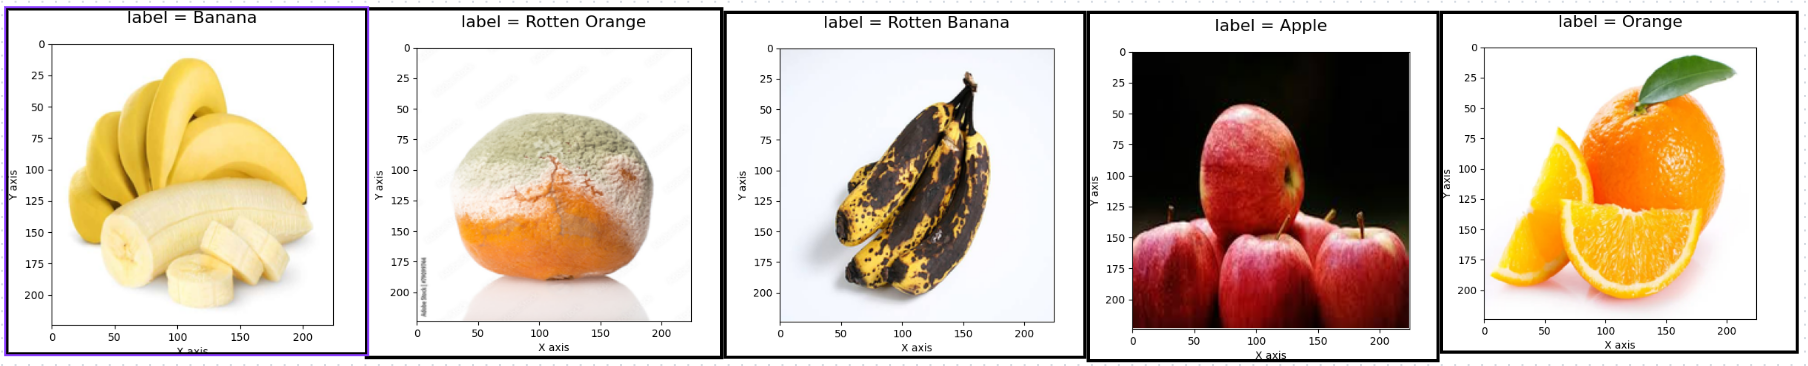
\includegraphics[width=\linewidth]{Example data.png}
    \caption{Example dataset.}
    \label{fig}
\end{figure}
\\
For the training dataset, the images are preprocessed through several steps. First, they are resized to a fixed size of 224x224 pixels. Then, random horizontal flipping is applied, which is a data augmentation technique to increase the diversity of training data. Next, the images are converted to PyTorch tensors, scaling the pixel values to the range [0, 1]. Finally, the images are normalized by subtracting the mean values [0.485, 0.456, 0.409] from each color channel (RGB) and dividing by the standard deviations [0.229, 0.224, 0.225].

For the test dataset, the preprocessing steps are similar but without the random horizontal flipping step. The images are resized to 224x224 pixels, converted to PyTorch tensors with pixel values scaled to [0, 1], and normalized using the same mean and standard deviation values as the training dataset. Consistent preprocessing between the training and test data is essential for accurate model evaluation and inference.

\section{Model Architecture}

The model makes use of structured learning during the training phase. Structured learning makes use of labels to train a model to preform classification tasks \cite{b1}. The labels used in this model are as follows: freshapples, freshbanana, freshoranges, rottenapples, rottenbanana, and rottenoranges.

The architecture of the model is as follows:
\begin{itemize}
    \item Input layer: Takes an input image of size (3, H, W), where 3 represents the RGB.
    \item Conv2d layers: Each convolutional layer is followed by a BatchNorm2d and ReLU activation.
    \item Dropout layer: Applied to avoid overfitting.
    \item Fully connected layers: the first linear layer reduces the flattened features, followed by a ReLU activation, and the second linear layer maps the features to the 6 output classes.
    \item Output layer: Provides the classification output for the 6 classes.
\end{itemize}

\begin{figure}[h]
    \centering
    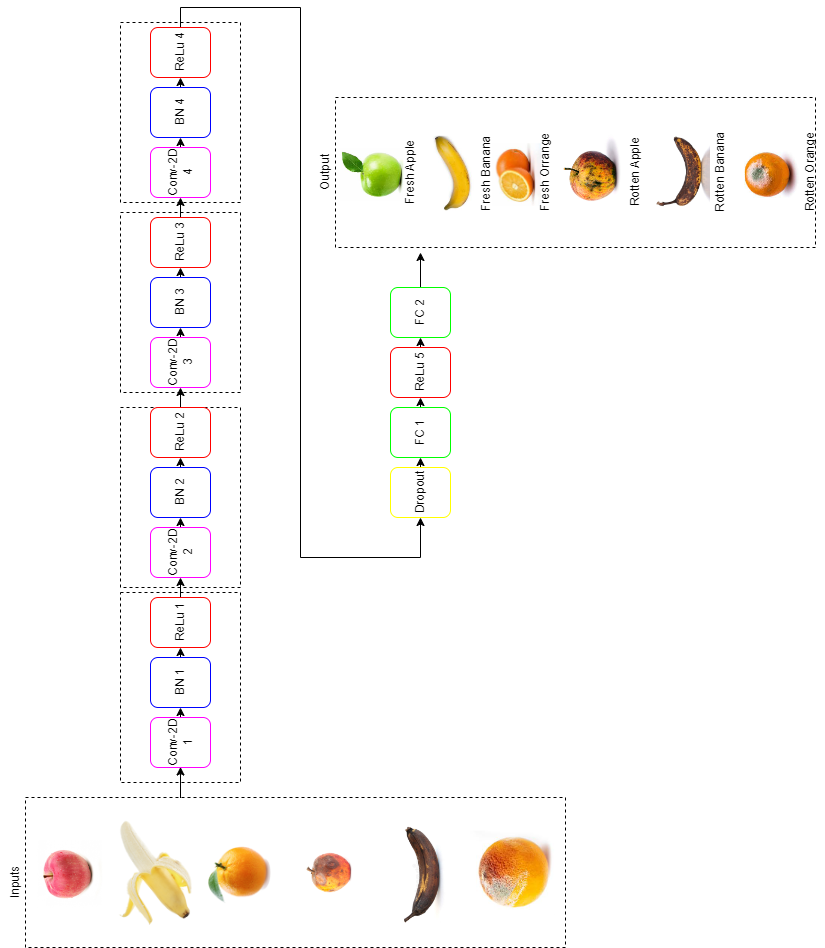
\includegraphics[width=\linewidth]{Ai Prent.drawio (1).png}
    \caption{Neural Network Architecture.}
    \label{fig}
\end{figure}

\begin{figure}[h]
    \centering
    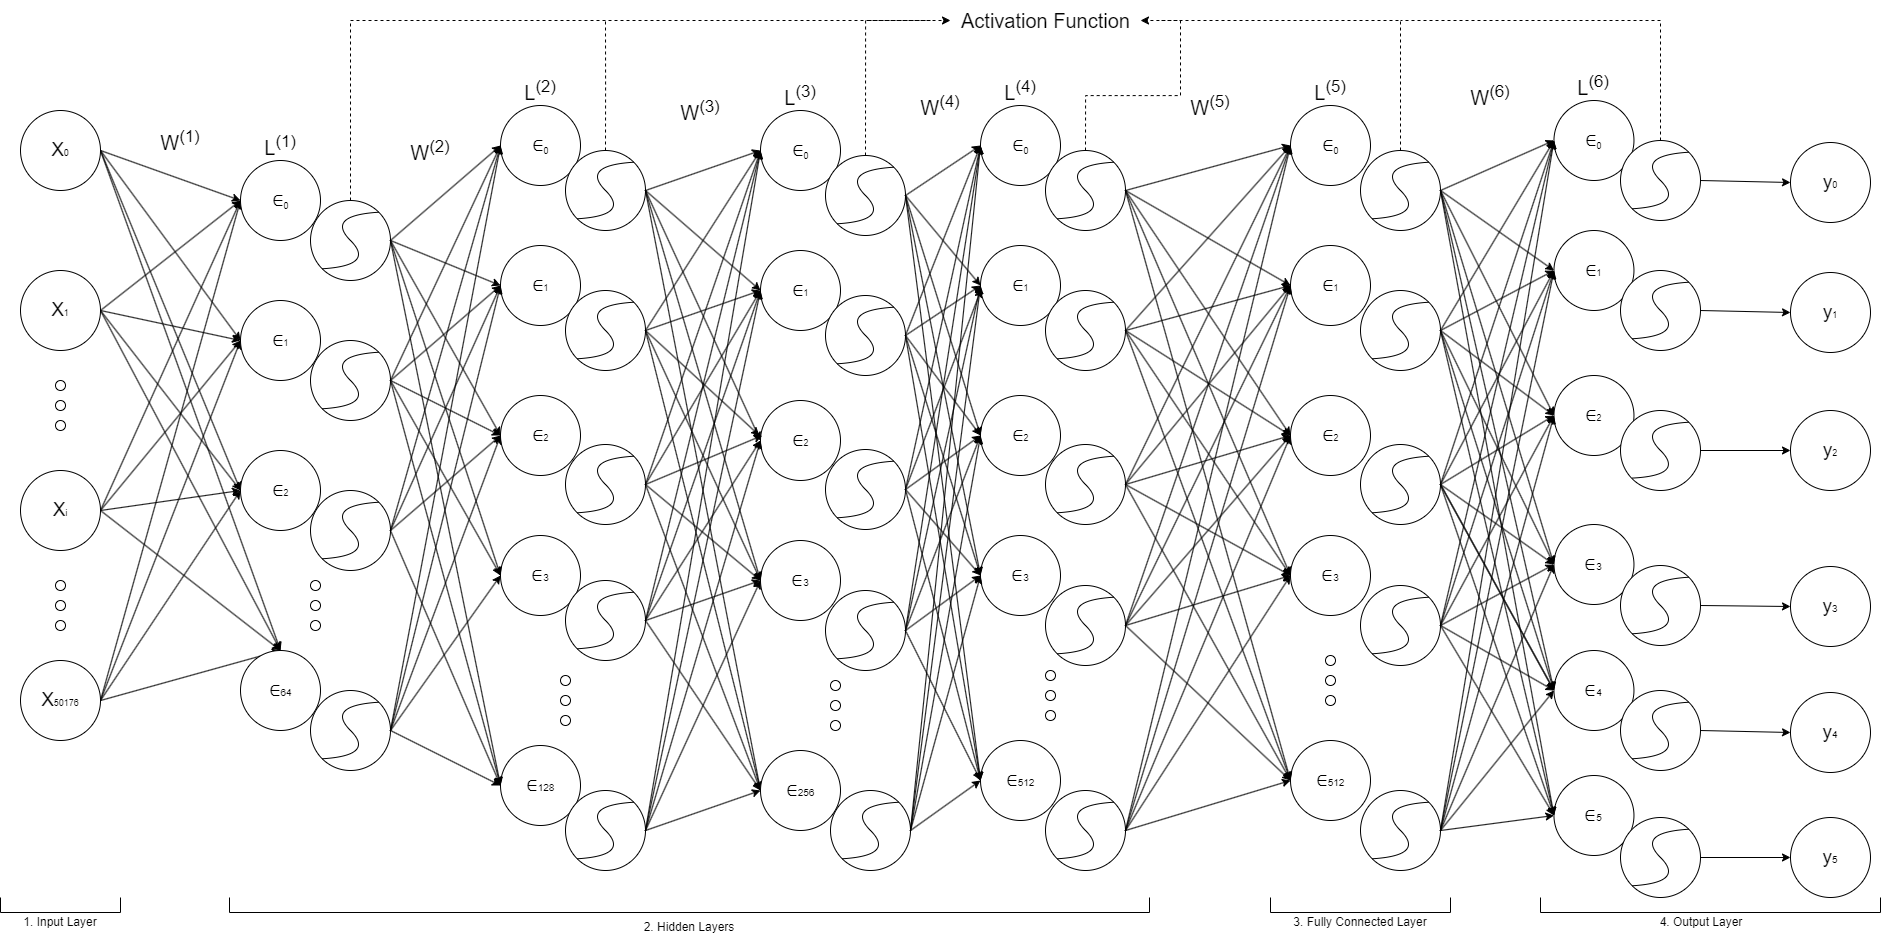
\includegraphics[width=\linewidth]{AI Architecture.drawio.png}
    \caption{Neural Network Architecture.}
    \label{fig}
\end{figure}

\subsection{Utilization of ReLU}
As ReLU, or rectified linear unit, can be effectively used in both pre-training and classification and is widely used in many applications.The structure of a deep network is complex, so it is hard to analyze the dynamics of learning process. Thus we study how complex networks need to be to approximate certain functions well. Where we optimize the trade-off between neural network complexity (measured by nonzero weights) and approximation fidelity for piecewise constant (or piecewise smooth) functions \cite{b1}.
\begin{figure}[h]
    \centering
    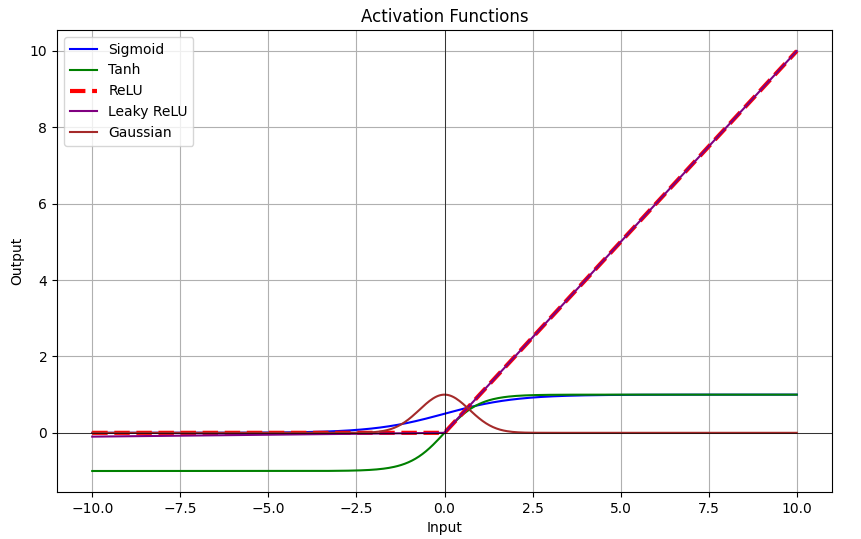
\includegraphics[width=\linewidth]{Activation Functions Compare.PNG}
    \caption{Activation Functions Comparison}
    \label{fig}
\end{figure}
\\
\\
The function is defined as
\textbf{\(f(x) = max(0,x)\)}
\\

Being computationally simple and efficient compared to other activation functions like sigmoid and tanh.Which means it requires only a thresholding at zero. This simplicity reduces the computational overhead during both the forward and backward passes of the network, speeding up the training process.

ReLU does not saturate in the positive domain. Unlike sigmoid or tanh, which can suffer from vanishing gradients due to their output being bounded between 0 and 1 or -1 and 1 respectively, ReLU outputs raw positive values. This helps in maintaining a strong gradient flow, especially in deeper networks, which facilitates faster convergence[Missing]

ReLU introduces sparsity by outputting zero for any input less than zero. This sparsity means that neurons are only activated for a subset of inputs, leading to a more efficient representation and reducing the risk of overfitting. Sparse activations also reduce the interdependence of neurons, making the model less likely to suffer from redundancy.[Missing]

ReLU is more biologically plausible compared to functions like sigmoid and tanh. It is similar to the firing rate of biological neurons, which are either active (firing) or inactive (not firing), rather than outputting a continuous range of values.[Missing]

ReLU has been empirically shown to perform well across a wide range of tasks and architectures. Many deep learning models that achieve state-of-the-art results in areas such as image recognition, natural language processing, and reinforcement learning use ReLU as the activation function.[Missing]

While sigmoid and tanh suffer from the vanishing gradient problem where gradients can become extremely small during backpropagation, leading to slow learning or even stagnation, ReLU helps mitigate this issue. In the positive range, the gradient of ReLU is always one, which helps maintain gradient magnitude.[Missing]

\section{Training Process}

The process of training the model went through different iterations.

With the first iteration we only had 1 convolutional layer with a batch size of 128 and the training was done on the CPU. This caused that the model would take longer to train, and the model was not accurate with classifying the if fruit are fresh or rotten. During the second iteration the model still had 1 convolutional layer but be lessened the batch size to 64 and the training was moved from the CPU to the GPU. A smaller batch size helps to increase the accuracy of an AI model \cite{b2} and helps prevent overfitting the model, and by moving the training from the CPU to the GPU we experienced a decrease in the time that it takes the model to train. But we still had a problem with the accuracy of the model.

The third iteration was the iteration where the amount of convolutional layers was increased from 1 to 4. This help to reduce the complexity of the model through the optimisation of each layer outputs \cite{b3}. For the forth iteration a Google Colab environment was used to train the model and the batch size was decreased to 32. By using Google Colab we were able to train the model by using a cloud base GPU. This allowed us to decrease the time that it toke the model to train.

The fifth iteration was the final iteration and for this iteration we changed the amount of epochs from 50 to 150. By changing the epoch the amount of time that the model will work through the training \cite{b4}. To avoid overfitting the AI model we added a patience variable.

\section{Experimentation and Results}

In order to create the final AI model that would is used in the application we preformed different experiments. These experiments include changing the epochs, changing the batch size, adding dropout layers, adding more convolutional layers, and adding a patience variable.

\subsection{Changing the Epochs}

With the first and second iterations of training the model the epoch was set to 20. From the third and forth iterations the epoch was set to 50. The fifth and final iteration the epoch was set to 150.

The epoch for the first and second iterations was chosen since it was the testing phase to find the best epoch for the model. For the third and forth iterations the epoch was set to 50 after reading \cite{b4} and testing, but the model was still not accurate. The final epoch for the fifth iteration was chosen since we wanted the model to train in one sitting, this was found to be the most effective epoch for training.

\subsection{Changing the Batch size}

The original batch size for training the model was 128. During the course of the iterative process of training the model the batch size was decreased to 64 and in the final iteration of training the model the batch size was decreased to 32.

This was done to increase the accuracy of the model after training, since by decreasing the batch size meant that the model would look at more images during the training process. Fig. 7 is a visual representation of how one of the batches look.

\begin{figure}[h]
    \centering
    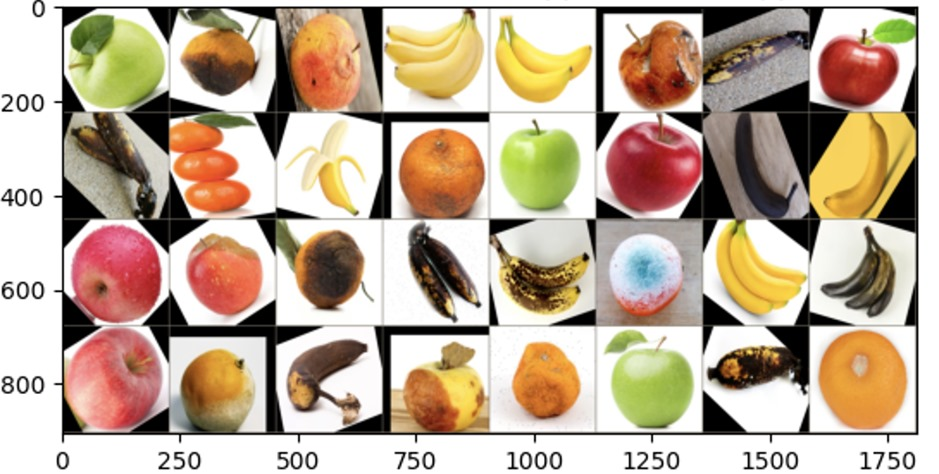
\includegraphics[width=\linewidth]{Batch_Representation.jpg}
    \caption{Visual Representation of a Batch}
    \label{fig}
\end{figure}

\subsection{More Convolutional Layers}

During the first 2 iterations of the training process our model only had 1 convolutional layer, this was done at first only to see if it is possible to create and train our own model. 

The third iteration was the first iteration where more layers were added. In this iteration the amount of convolutional layers went form 1 to 4 layers, this was done to increase the accuracy of the model by reducing the complexity of the convolutional network \cite{b3}.

\subsection{Adding Dropout Layers}

Before third iteration of the training process, the model did not have a dropout layer. The dropout layer was only added in the third iteration of the training process.

The dropout layer was added to avoid overfitting the model. The dropout layer works by removing neurons from the network based on their activation \cite{b5}. If the activation of a neuron in the network is greater than our dropout value, which is 0.5, the likelihood of deactivating the neuron is increased.

\subsection{Adding a Patience Variable}

Since the epoch for the training of the model was 50 or less we did not add a patience variable, but since with the fifth and final iteration with the epoch set to 150 it was needed to add a patience variable, to ensure that once the model reached a state where there was no longer any improvement the model would stop training.

The patience variable for the training of the model was set to 10. And to measure if the model was improving we add a loss function. The loss was calculated by dividing the running loss of the epoch by the size of the train dataset. The lower the loss value the more accurate the model is, and this value is saved as the best loss value. In order for the patience variable to take effect the best loss value would have to be the same for 10 epochs. If the best loss value staid the same for the 10 epochs the model would stop training. Since if the model would continue training after no impairments where made there would be a chance that the model could be overfitted \cite{b5}. Fig. 5 shows how the loss value decreased with each epoch.

\begin{figure}[h]
    \centering
    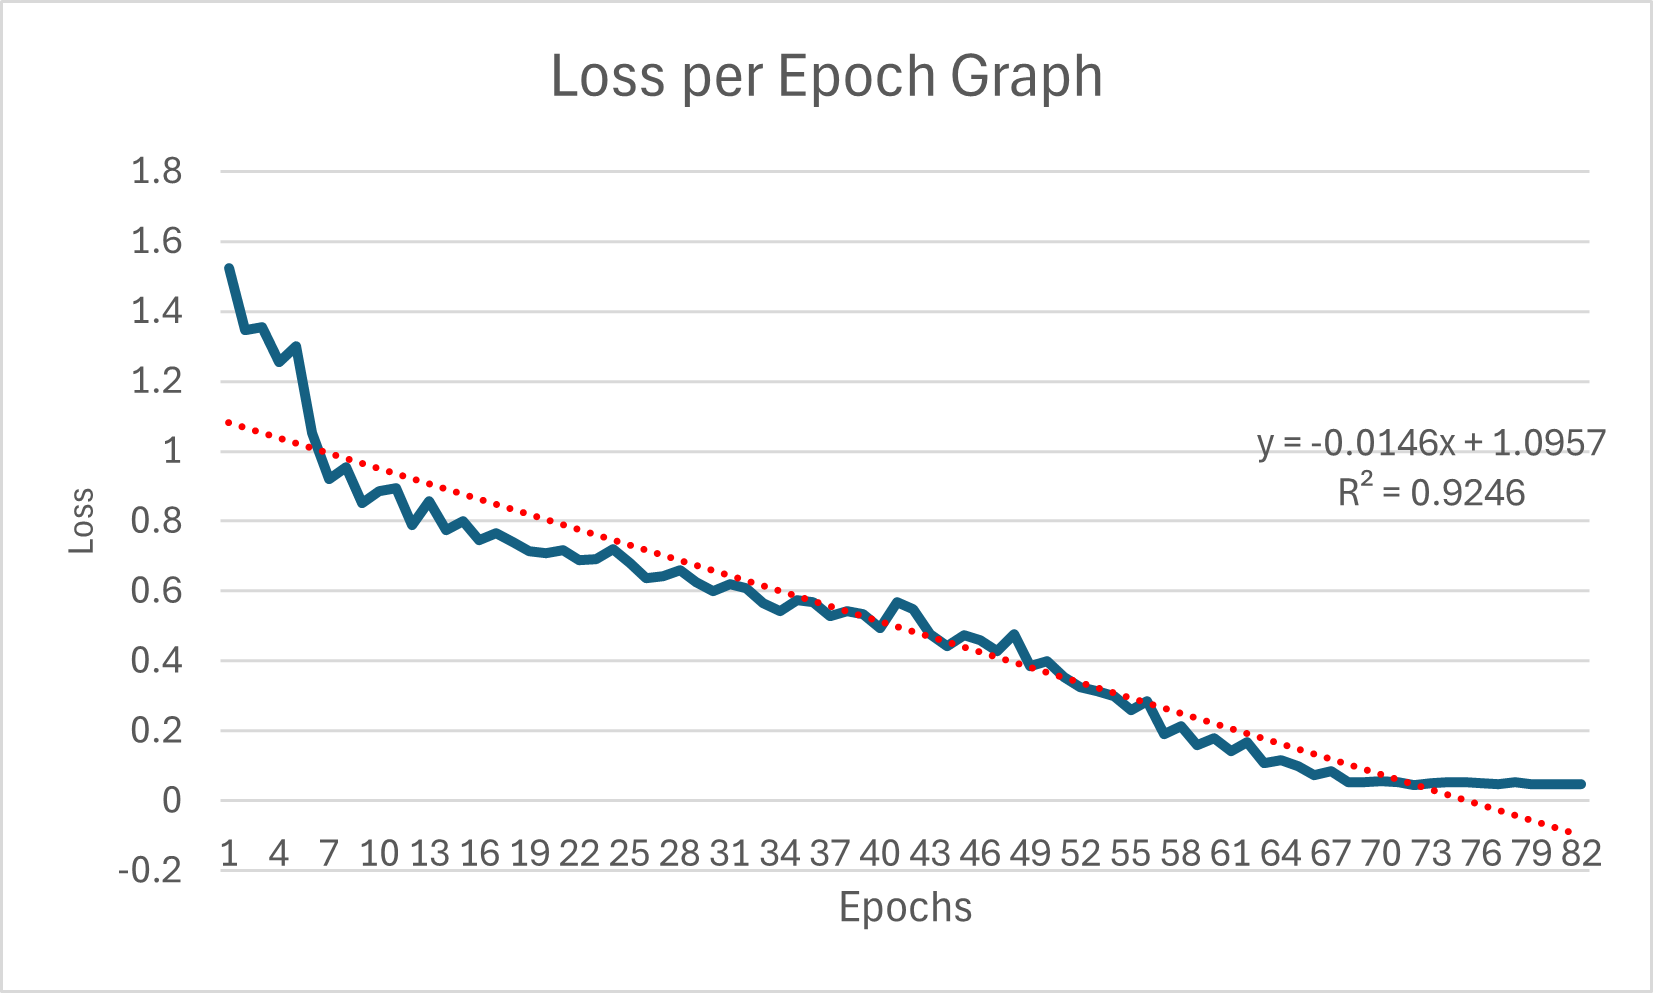
\includegraphics[width=\linewidth]{Loss_per_Epoch_Graph.png}
    \caption{Loss per Epoch.}
    \label{fig 3}
\end{figure}

\section{Conclusion}

\section*{Acknowledgment}

We would like to acknowledge Pieter Swanepoel for assisting us with the setup of the Google Colabe environment.

% \section*{References}

% Please number citations consecutively within brackets \cite{b1}. The 
% sentence punctuation follows the bracket \cite{b2}. Refer simply to the reference 
% number, as in \cite{b3}---do not use ``Ref. \cite{b3}'' or ``reference \cite{b3}'' except at 
% the beginning of a sentence: ``Reference \cite{b3} was the first $\ldots$''

% Number footnotes separately in superscripts. Place the actual footnote at 
% the bottom of the column in which it was cited. Do not put footnotes in the 
% abstract or reference list. Use letters for table footnotes.

% Unless there are six authors or more give all authors' names; do not use 
% ``et al.''. Papers that have not been published, even if they have been 
% submitted for publication, should be cited as ``unpublished'' \cite{b4}. Papers 
% that have been accepted for publication should be cited as ``in press'' \cite{b5}. 
% Capitalize only the first word in a paper title, except for proper nouns and 
% element symbols.

% For papers published in translation journals, please give the English 
% citation first, followed by the original foreign-language citation \cite{b6}.

\begin{thebibliography}{00}
\bibitem{b1} Niculescu-Mizil, A. and Caruana, R., 2007, March. Inductive transfer for Bayesian network structure learning. In Artificial intelligence and statistics (pp. 339-346). PMLR.
\bibitem{b2} McCandlish, S., Kaplan, J., Amodei, D. and Team, O.D., 2018. An empirical model of large-batch training. arXiv preprint arXiv:1812.06162.
\bibitem{b3} O'shea, K. and Nash, R., 2015. An introduction to convolutional neural networks. arXiv preprint arXiv:1511.08458.
\bibitem{b4} Brownlee, J., 2018. What is the Difference Between a Batch and an Epoch in a Neural Network. Machine learning mastery, 20.
\bibitem{b5} Santos, C.F.G.D. and Papa, J.P., 2022. Avoiding overfitting: A survey on regularization methods for convolutional neural networks. ACM Computing Surveys (CSUR), 54(10s), pp.1-25.
\bibitem{b6} Gu, J. et al., 2018. Recent advances in convolutional neural networks. Pattern Recognition, Volume 77, pp. 354-377.
\bibitem{b7} Kazuyuki, H., Daisuke, S. , Hayaru Shouno, 2015. Analysis of function of rectified linear unit used in deep learning. In: 2015 International Joint Conference on Neural Networks. s.l.:s.n., pp. 1-8.
\end{thebibliography}

\end{document}